% document's head

\begin{center}
    \LARGE \textsc{Лабораторная работа № 6.11.1} \\
    \vspace{3 mm}
    \large Закон Кюри-Вейсса и обменное взаимодействие в ферромагнетиках
\end{center}

% \hrule

\phantom{42}

\begin{flushright}
    \begin{tabular}{rr}
    % written by:
        % \textbf{Источник}: 
        % & \href{__ссылка__}{__название__} \\
        % & \\
        % \textbf{Лектор}: 
        % & _ФИО_ \\
        % & \\
        \textbf{Автор работы}: 
        & Хоружий Кирилл \\
        & \\
    % date:
        \textbf{От}: &
        \textit{\today}\\
    \end{tabular}
\end{flushright}

\thispagestyle{empty}

\vspace{10mm}


\subsection*{Цель работы}
\begin{enumerate*}
    \item Исследовать температурную зависимость проводимости полупроводника.
    \item Определить ширину запрещенной зоны полупроводника из полученной зависимости.

\end{enumerate*}


\vfill

\begin{figure}[h]
    \centering
    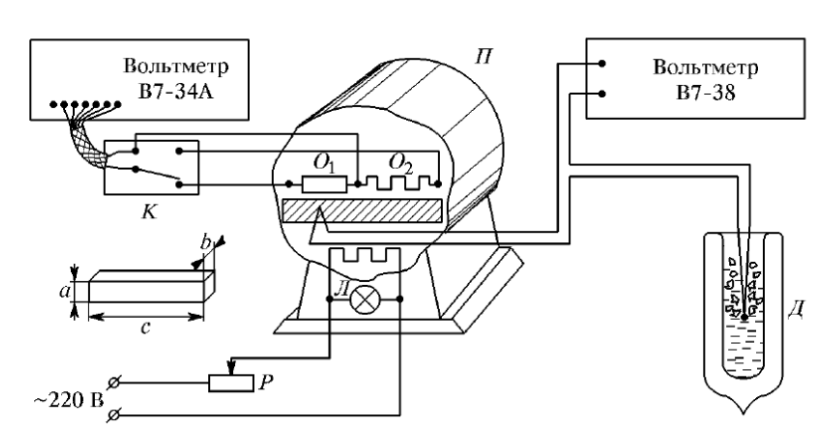
\includegraphics[width=0.5\textwidth]{exp.png}
    \caption{Схема установки}
    \label{fig:exp}
\end{figure}


\subsection*{Оборудование}

Схема установки, используемой в работе, приведена на рисунке \ref{fig:exp}. Исследуемые образцы O$_1$ и O$_2$ помещены в электронагревательную печь П; их сопротивление изменяется вольтметром В7-34А. Абсолютную погрешность измерений сопротивления примем равной $2\cdot10^{-4}$ кОм. 
    

Полупроводниковый образец имеет форму параллелепипеда, его параметры: $4.0 \times 4.0 \times 39$ (в мм). Медный образец - тонкая проволока длиной $l = 20$ м диаметра $d = 0.05$ мм.

Удельная проводимость $\sigma$ связана с измеряемым сопротивлением $R$ следующей формулой: 




Температура образцов измеряется с помощью термопары, один спай которой расположен в печи, а другой - в сосуде Дьюара Д. 
